\documentclass[10pt]{article}
\usepackage{icmlko}

\icmlmeta{IP 파운데이션 월드모델}{278}{판이 고른 것}{정식화 일곱에 같은 열을 줘 봤다 --- 판 상위 셋이 전부 작은 도메인의 전용 정보에 눈이 멀어 있다}

\begin{document}

\twocolumn[
\icmlheader

\begin{abstract}
노트 277이 F21 능형과 F18 나무에서 갈렸고, 판 $\rho$ 는 그 갈림을 못 본다.
그래서 손으로 표를 만들었다 --- 정식화 일곱에 팝업(관측 학습 \textbf{14행})
전용 열로 \textbf{라벨 순위를 그대로} 주고 쓸 수 있는지 쟀다. \textbf{눈이
머는 방식이 셋이다}: 잎 하한(F8 · F18, $+$0.0000) · 도메인별 배합(F10
$+$0.0000 · F21 $+$0.0880) · 그리고 안 머는 쪽인 순수 풀링(F6 $+$0.5272 ·
F9 $+$0.6341). \textbf{노트 277의 ``능형 대 나무''는 너무 거친 틀이었다} ---
F10은 선형인데 정확히 0 이고 F6도 선형인데 0.53 이다. 가르는 것은 선형이냐가
아니라 \textbf{그 도메인의 열을 계수로 푸느냐, 아니면 남에게서 빌려 오느냐}다.
F23 섞음이 검산을 해 준다 --- F21과 F18의 반반 순위 평균이니 예측이
$(0.0880{+}0)/2 = 0.0440$ 인데 잰 값이 \textbf{$+$0.0454} 다. 남는 것이
불편하다: \textbf{판 상위 셋(F23 · F18 · F8)이 전부 $|$이득$| \le 0.0454$
이고, 전용 정보를 온전히 쓰는 둘(F6 · F9)은 다섯째 · 여섯째다.} 다만
\textbf{순위 상관은 $-$0.34(n${=}$7, p${=}$0.46)로 유의하지 않고}, F10이
판도 꼴찌면서 못 쓰는 \textbf{반례}다 --- ``눈이 멀면 판에서 이긴다''는
아니다. 지금 말할 수 있는 것은 \textbf{현재 포트폴리오의 상태}이지 법칙이
아니다. 그래도 그 상태가 문제다 --- 이 실험실의 목표가 IP 파운데이션이고,
파운데이션은 작은 도메인에 쓰라고 만드는 것이다.
\end{abstract}
]

\section{판이 못 보는 성질을 손으로 잰다}

노트 277이 남긴 줄 하나가 ``정식화 성질표 --- 판이 못 보는 성질을 따로 적어
둘 것''이었다. 그것을 했다.

\textbf{눈금은 하나다.} 팝업에 \textbf{라벨 순위를 그대로} 전용 열로 준다.
이보다 센 열은 없으니, 이 열로 못 오르면 그 정식화는 팝업의 전용 정보를
\emph{원리적으로} 못 쓰는 것이다. 문턱 15 · 씨앗 0 · 축 23에 한 열을 더한
판이다. \textbf{진단 전용이고 채택은 없다.}

\begin{figure*}[t]
\centering
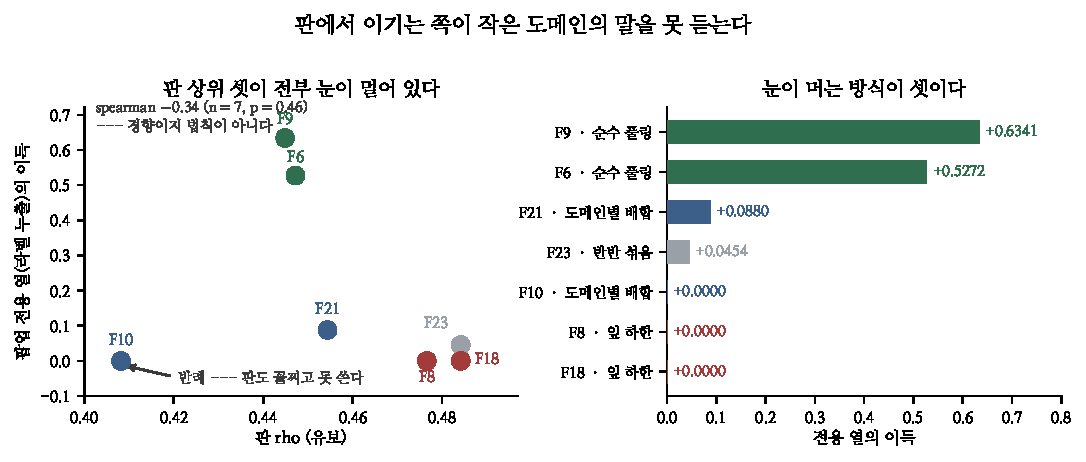
\includegraphics[width=\textwidth]{figs/picked.pdf}
\caption{왼쪽 --- 판 $\rho$ 와 팝업 전용 열(라벨 누출)의 이득. 오른쪽 ---
같은 값을 기전별로 세운 것. 색은 기전이다(초록 순수 풀링 · 파랑 도메인별
배합 · 붉은 잎 하한 · 회색 반반 섞음).}
\end{figure*}

\begin{center}\small
\begin{tabular}{lrrl}
\hline
정식화 & 판 $\rho$ & 이득 & 기전 \\
\hline
F9\_ranklik & 0.4449 & \textbf{$+$0.6341} & 순수 풀링 \\
F6\_directpool & 0.4472 & \textbf{$+$0.5272} & 순수 풀링 \\
F21\_recentpick & 0.4544 & $+$0.0880 & 도메인별 배합 \\
F23\_rankmix & \textbf{0.4842} & $+$0.0454 & 반반 섞음 \\
F10\_pershrink & 0.4082 & $+$0.0000 & 도메인별 배합 \\
F8\_boost & 0.4766 & $+$0.0000 & 잎 하한 \\
F18\_bagboost & \textbf{0.4842} & $+$0.0000 & 잎 하한 \\
\hline
\end{tabular}
\end{center}

\section{노트 277의 틀이 거칠었다}

어제 ``능형은 쓰고 나무는 못 쓴다''고 적었다. \textbf{이 표가 그걸
정정한다.}

\begin{center}\small
\begin{tabular}{lll}
\hline
& 선형인가 & 이득 \\
\hline
F6\_directpool & 예 & $+$0.5272 \\
F9\_ranklik & 예 & $+$0.6341 \\
\textbf{F10\_pershrink} & \textbf{예} & \textbf{$+$0.0000} \\
\hline
\end{tabular}
\end{center}

\textbf{선형이면서 정확히 0 인 것이 있다.} 그러니 가르는 것은 선형/비선형이
아니다. 표를 기전으로 다시 묶으면 이렇게 된다.

\begin{itemize}
\item \textbf{순수 풀링}(F6 · F9) --- 전 도메인을 한 표로 놓고 계수를 푼다.
팝업 14행짜리 열도 제 계수를 받는다. \textbf{쓴다.}
\item \textbf{도메인별 배합}(F10 · F21) --- 도메인마다 ``제 이력 대 남의
이력''의 비를 따로 정한다. 팝업처럼 제 이력이 얇으면 배합이 남 쪽으로
쏠리고, \textbf{남에게는 그 열이 없다}(마스크 0). 그래서 전용 열이 통째로
버려진다. F10은 완전히($+$0.0000), F21은 일부만($+$0.0880).
\item \textbf{잎 하한}(F8 · F18) --- 노트 276이 판 것. 관측 14행으로는 어느
쪽 잎도 \texttt{min\_samples\_leaf}$=$20 을 못 채워 분기가 후보에도 못
오른다. \textbf{정확히 0.}
\end{itemize}

\paragraph{검산이 맞는다} F23\_rankmix 는 정의상 F21과 F18의 반반 순위
평균이다. 예측은 $(0.0880 + 0.0000)/2 = 0.0440$ 이고 잰 값이 \textbf{$+$0.0454}
다. \textbf{기전 분해가 산수로 닫힌다} --- 눈이 머는 정도가 섞으면 섞이는
양이라는 뜻이고, 노트 250이 ``전용 이름은 가법''이라 한 것의 다른 자리에서의
확인이다.

\section{불편한 줄, 그리고 그 줄의 한계}

표를 판 순으로 세우면 이렇다.

\begin{center}\small
\begin{tabular}{lrr}
\hline
판 순위 & 정식화 & 이득 \\
\hline
1 & F23\_rankmix 0.4842 & $+$0.0454 \\
1 & F18\_bagboost 0.4842 & $+$0.0000 \\
3 & F8\_boost 0.4766 & $+$0.0000 \\
4 & F21\_recentpick 0.4544 & $+$0.0880 \\
5 & F6\_directpool 0.4472 & $+$0.5272 \\
6 & F9\_ranklik 0.4449 & $+$0.6341 \\
7 & F10\_pershrink 0.4082 & $+$0.0000 \\
\hline
\end{tabular}
\end{center}

\textbf{판 상위 셋이 전부 눈이 멀어 있고, 온전히 보는 둘이 다섯째 ·
여섯째다.}

\paragraph{여기서 멈춰야 한다} 순위 상관은 \textbf{$-$0.337 (n${=}$7,
p${=}$0.46)} 로 \textbf{유의하지 않다.} F10을 빼면 $-$0.868(p${=}$0.025)이
되는데 \textbf{그 제외는 사후다} --- 이 실험실은 그 함정에 이미 한 번
빠졌고(더현대 ``22$\sim$47\%''가 체리피킹이었다) 규약이 ``부분집합 주장엔
반드시 제외 기준 명시''다. 그래서 헤드라인은 \textbf{$-$0.34, 유의하지
않음}이다.

그리고 F10이 진짜 반례다 --- \textbf{판도 꼴찌(0.4082)면서 못 쓴다.} 눈이
머는 것이 판을 벌어 주는 게 아니다. 기전을 보면 당연하다: F10의 실명은
배합이 남 쪽으로 쏠려서인데, 그 쏠림은 판도 같이 깎는다.

\textbf{그러니 ``판정치가 실명을 선택했다''고는 못 쓴다.} 쓸 수 있는 것은
이것뿐이다 --- \textbf{지금 포트폴리오의 상위권이 마침 전부 눈이 멀어 있고,
판 $\rho$ 는 그 사실을 한 번도 보고한 적이 없다.}

\section{그래서 왜 문제인가}

이 실험실의 목표는 IP 파운데이션 월드모델이다. 파운데이션이 값을 하는
자리는 \textbf{자료가 얇은 도메인}이다 --- 두꺼운 도메인은 제 모형을
따로 만들면 된다(노트 252가 잰 대로 아홉 중 다섯은 여지가 이미 음수라
전용 모형이 풀링보다 나쁘다).

그런데 우리가 챔피언을 고르는 눈금은 유보 표본 크기로 가중한 판 $\rho$ 이고,
그 눈금에서 \textbf{팝업은 2.3\% · 아이돌은 1.0\%}다. 노트 274가 잰 대로
팝업에서 도메인 안 $\Delta\rho{=}0.435$ 가 있어야 판이 겨우 반응한다.
\textbf{얇은 도메인을 잘 다루는 능력은 판정치에 실리지 않는다.} 오늘 표가
그것을 구체적인 성질 하나로 보여 준 것이다.

\paragraph{바꾸자는 게 아니다} 노트 268의 규약이 있다 --- \textbf{판정 눈금을
바꾸자는 제안이 나오면 먼저 두 눈금으로 줄을 세워 보고, 순위가 같으면 안
바꾼다.} 그리고 노트 277이 확인했듯 \textbf{지금 팝업에 쓸 전용 정보 자체가
없다}(진짜 축 넷은 능형에서도 $-$0.0070). 바꿀 근거는 아직 없다.

바뀌는 것은 \textbf{기록}이다. 판 $\rho$ 옆에 이 열을 같이 적는다.

\paragraph{남은 것}
\begin{center}\small
\begin{tabular}{ll}
\hline
갈래 & 왜 \\
\hline
성질표를 루프에 & 승격 때 이 열도 같이 적기 \\
아이돌 54행 & 벼랑 바로 위 --- 기전 셋이 거기선? \\
배합 쏠림 직접 재기 & F10 · F21의 팝업 배합비를 꺼내 볼 것 \\
큰 도메인에서도 재기 & 웹툰 전용 열은 일곱 다 쓰나 \\
\hline
\end{tabular}
\end{center}

\paragraph{규약} \textbf{판정치가 못 보는 성질은 판정치 옆에 손으로 적는다.}
그리고 \textbf{기전으로 묶기 전에 반례를 찾는다} --- 오늘 ``선형이면 쓴다''를
쓸 뻔했고 F10이 막았다. 노트 277이 하루 만에 좁혀진 데 이어 이틀째다.

\end{document}
